\section{First version of Cauchy's theorem}
\lecture{4}{22/1}

\begin{definition}[]
    A domain $D$ is \textbf{starlike} if there exists $a_0 \in D$
    such that for all $b \in D$, the line segment from $a_0$ to $b$
    is in $D$.
\end{definition}

\begin{example}
    $\C$ and $B_r(a)$ are starlike. $\C^\star$ is \emph{not} starlike.
\end{example}

\begin{theorem}[Cauchy's theorem for starlike domains]
    Let $D \subset \C$ be a starlike domain
    and $f: D \to \C$ be holomorphic.
    Then for any closed contour $\gamma \subset D$
    \[
        \int_\gamma f(z) \, dz = 0.
    \]
\end{theorem}

The same is true on $f$ being continuous on $D$
and holomorphic on $D \setminus S$ for some finite set $S$.

\begin{lemma}[]
    Let $U$ be an open set, $f: U \to \C$ be holomorphic, 
    and $\triangle \subset U$ be a triangle in $U$.
    Then
    \[
        \int_{\partial\triangle} f(z) \, dz = 0.
    \]
\end{lemma}

As a technical aside, the same also holds for $f$ being holomorphic on 
$U \setminus S$ for some finite set $S$.
This point is important in a later proof.

\begin{figure}[]
    \centering
    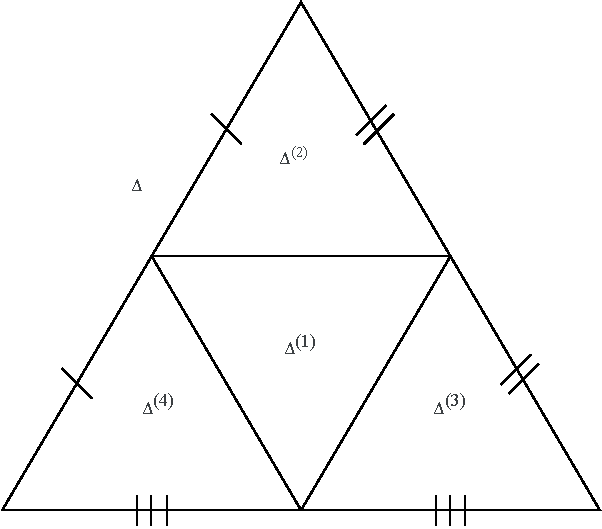
\includegraphics[width=0.5\linewidth]{images/triangulation-cauchy.pdf}
    \caption{Triangulation method for proof of Cauchy's theorem for starlike domains.}
    \label{fig:triangulation-cauchy}
\end{figure}

\begin{proof}
    With regard to the technical aside, we will take 
    $S = \varnothing$.
    Here we subdivide $\triangle$ into for smaller triangles
    $\triangle^{(1)}$, $\triangle^{(2)}$, $\triangle^{(3)}$, and $\triangle^{(4)}$.
    As these triangles are similar, we have
    \[
        L\left(\partial \triangle^{(i)}\right) = \frac12 L(\partial \triangle).
    \]
    Now we claim that
    \[
        \int_{\partial \triangle} f(z) \, dz
        = \sum_{i} \int_{\partial \triangle^{(i)}} f(z) \,dz \tag{$\star$}.
    \]
    This is because the internal sides that are covered twice and
    traversed both anticlockwise then clockwise; hence,
    they cancel out.
    \[
        (\star) \implies 
        \left\lvert 
        \int_{\partial \triangle} f(z) \,dz 
        \right\rvert
        \leq \sum_{i} 
        \left\lvert 
            \int_{\partial \triangle^{(i)}} f(z) \,dz 
        \right\rvert
        .
    \]
    Now let $\triangle_1 = \triangle^{(i)}$ such that
    $\left\lvert \int_{\partial \triangle^{(i)}} f(z) \,dz \right\rvert$
    is maximal.
    Now
    \[
        \left\lvert
            \int_{\partial \triangle} f(z) \,dz
        \right\rvert
        \leq 4
        \left\lvert
            \int_{\partial \triangle_1} f(z) \,dz
        \right\rvert
        .
    \]
    Note that we also have $L(\partial \triangle_1) = \frac12 L(\partial\triangle)$.
    We now repeat this procedure to get
    \[
        \left\lvert
            \int_{\partial \triangle} f(z) \,dz
        \right\rvert
        \leq 4^2
        \left\lvert
            \int_{\partial \triangle_2} f(z) \,dz
        \right\rvert
    \]
    where $L(\partial \triangle_2) = \frac1{2^2} L(\partial\triangle)$
    and $\triangle_2 \subset \triangle_1 \subset \triangle$.
    We keep repeating this to get
    \[
        \triangle \supset \triangle_1 \supset \triangle_2 \supset \ldots
        \supset \triangle_n \supset \ldots
    \]
    and so
    \[
        \left\lvert 
            \int_{\partial\triangle} f(z) \,dz
        \right\rvert
        \leq
        4^n
        \left\lvert
            \int_{\partial \triangle_n} f(z) \,dz
        \right\rvert
    \]
    and $L(\partial \triangle_n) = \frac1{2^n} L(\partial \triangle)$.
    Let $w = \bigcap_{n = 1}^\infty \triangle_n$ and
    \[
        g(z) =
        \begin{cases}
            \frac{f(z) - f(w)}{z - w} - f'(w) & z \neq w \\
            0 & z = w. \\
        \end{cases}
    \]
    $g$ is continuous on $U$ since $f$ has a derivative at $w$ and
    holomorphic in general.
    Then
    \[
        f(z) = f(w) + (z- w)f'(w) + g(z)(z - w)
    \]
    and so
    \begin{align*}
        \int_{\partial \triangle_n} f(z) \,dz
        &= \int_{\partial\triangle_n} 
            \left( f(w) + (z - w) f'(w) + g(z)(z - w) \right) \,dz \\
        &= \int_{\partial\triangle_n} g(z)(z - w)\,dz
    \end{align*}
    as there exists an antiderivative for $f(w) + (z-w)f'(w)$
    and hence it is 0.  %hmmm?
    \begin{align*}
            \left\lvert
                \int_{\partial\triangle} f(z) \,dz
            \right\rvert
        &\leq 4^n
            \left\lvert 
                \int_{\partial\triangle_n} f(z) \,dz
            \right\rvert
            \\
        &= 4^n
            \left\lvert
                \int_{\partial\triangle_n} (z - w) g(z) \,dz
            \right\rvert
                \\
        &\leq 4^n L(\partial\triangle_n) 
            \sup_{\partial\triangle_n} 
            \left(
                \lvert z - w \rvert 
                \lvert g(z) \rvert
            \right)
            \\
        &\leq 4^n L(\partial\triangle_n) \sup_{\partial\triangle_n} \lvert g(z) \rvert
            \\
        &= 4^n \left( \frac{L(\partial\triangle)}{2^n} \right)^2
            \sup_{\partial\triangle_n} \lvert g(z) \rvert \\
        &= L(\partial\triangle)^2 \sup_{\partial\triangle_n} \lvert g(z) \rvert
            \to 0
    \end{align*}
    as $n \to \infty$.
    As $g$ is continuous, $g(w) = 0$, and $\triangle_n$ converges to $w$ as
    $n \to \infty$
    then 
    \[
        \int_{\triangle} f(z) \,dz = 0
    \]
    by squeezing.
\end{proof}
